\documentclass[UTF8, zihao = -4, linespread = 1.335, heading = true, fontset = none]{ctexart}
\usepackage{ujnthesis}

\begin{document}

%
%   毕业论文文档装订顺序(据信息学院 2018.6.2 更新版本):
%
%   1 毕业论文(设计)(封皮)                  // 计科计卓计软统一专业名:计算机科学与技术
%   2 毕业论文(设计)正文
%   3 毕业论文(设计)附件(封皮)
%   4 毕业论文(设计)任务书
%   5 毕业论文开题报告/毕业设计方案
%   6 毕业论文(设计)外文资料翻译(封皮)       // 此处的题目是翻译的文章的中文题目
%   7 英文原文
%   8 英文译文
%
%   // 以下文档由学生提交电子版,后期老师的评语和评分统一打印,签字和日期必须手写
%
%   9-1 毕业论文(设计)开题评分表
%   9-2 毕业论文(设计)中期检查评分表
%   9-3 毕业论文(设计)日常考核评分
%   9-4 毕业论文(设计)评阅评分表
%   9-5 毕业论文(设计)答辩评分表
%   10 毕业论文(设计)评语
%


        %%%%%%%%%%%%%%%%%%%%%%%%%%%%%%%%%%%%%%%%%%%%%%%%%%%%%%%%
        %%%%%%     下列 非 毕业论文正文部分,请按需包含       %%%%%
        %%%%%%%%%%%%%%%%%%%%%%%%%%%%%%%%%%%%%%%%%%%%%%%%%%%%%%%%


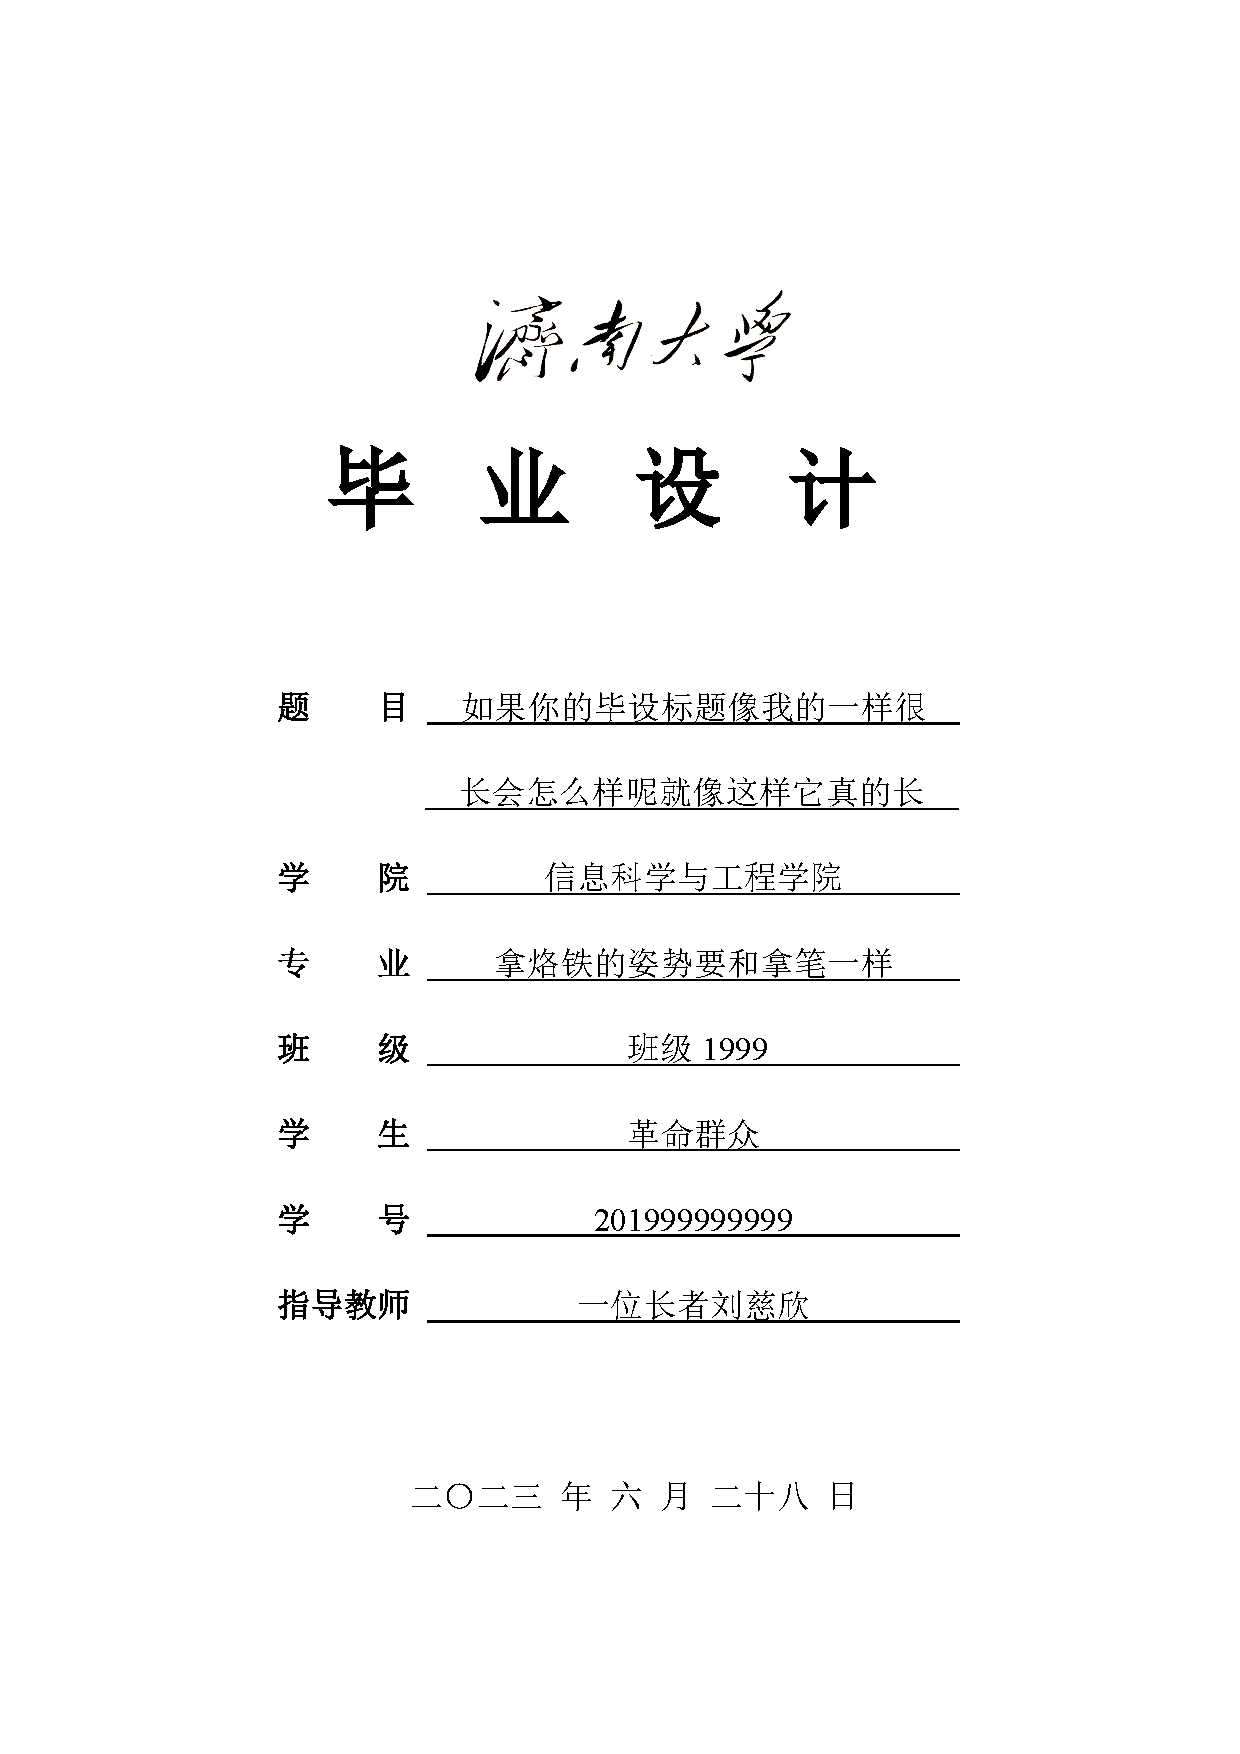
\includepdf[pages=-]{docs/01-cover.pdf}                     % 1 毕业论文封面

%%%%%%%%%%%%%%%%%%%%%%%%%%%%%% 毕业论文正文 %%%%%%%%%%%%%%%%%%%%%%%%%%%%%%%%%

\setblindingline
\setfancylength
\pagestyle{ujnabstract}
\begin{ujnabstract}
\section[摘要]{摘\qquad 要}
% 以下为中文摘要,把点引线以下的文字替换成你的就好
% ·································································································
近日,由教务处 教学质量与评估办公室编写的《“四路并举”赋能专业建设新样态》成功入选教育部《全国普通高校本科教育教学质量报告》(以下简称《质量报告》)应用典型案例,
并将编入由高等教育出版社出版的《数智助鉴 以鉴促强——落实质量主体责任高校在行动》一书。

《质量报告》是在教育部教育督导局指导下,由教育部教育质量评估中心会同有关高校、
教育研究机构等单位组建的学术团队联合研制,系统反映我国普通高校本科教育教学质量发展状况的年度报告。
应用案例征集活动旨在选树一批高校教学质量管理优秀典型,巩固本科教育教学改革成果,完善体制机制建设。

入选案例《“四路并举”赋能专业建设新样态》系统总结了学校近年来深化专业综合改革的建设举措以及成效。
以“需求驱动、质量带动、产业拉动、内外联动”为引擎,围绕“四新”专业建设主线,推动本科专业供给侧改革,
优化专业布局动态调整,积极搭建产教融合育人平台,持续推进专业建设高水平发展,提高专业人才培养质量。

近年来,学校高度重视本科教育教学工作,始终坚持以习近平新时代中国特色社会主义思想为指导,
落实立德树人根本任务,推动学校本科教育内涵建设和高质量发展。学校将充分学习和研究《质量报告》,
进一步扎实做好本科教育教学质量常态监测、编制发布本科教学质量报告和专业人才培养状况报告等工作。
以数据分析报告为重要依据,积极引导各专业明确定位、强化特色、加强优势、提升质量,构筑高水平人才培养体系,
不断提升育人成效。
% ·································································································
% 以下为关键词的设置,把「关键词n」(n=1,2,3,...)替换成你的关键词就好
\small\cnkeywords{祝贺;这就是;济大}
\end{ujnabstract}
                 % 2.1 中文摘要
\pagestyle{ujnabstract*}
\begin{ujnabstract*}
\section{ABSTRACT}
\begin{spacing}{1.4}\normalsize{
% 以下为英文摘要,把点引线以下的文字替换成你的就好
% ·································································································
The University has established 4 national-level distinctive specialties,
5 national-level quality courses, 2 national-level exemplary bilingual courses,
2 national-level quality public audio and video courses,
6 specialties training for Outstanding Engineers, 16 provincial-level distinct specialties,
9 specialties jointly supported by the school and enterprise,
53 provincial-level top-grade courses and 5 provincial-level experimental teaching centers.
In recent years, the faculties have undertaken 6 national teaching and research projects and 55 provincial projects,
published 8 textbooks guided by China, and won 3 national "Teaching Achievements" awards and 75 provincial "Teaching and Research Achievements" awards.
In addition, the University has successively won a wide variety of honors for innovation and creativity,
such as the "Challenge Cup" Extracurricular and Academic Contest,
and China Undergraduate Mathematical Contest in Modeling.
The students have won 3133 provincial or national awards,
of which 48 are first prizes and 125 are second prizes at the national level.

In recent years, the university has undertaken 347 national research projects including funds from the National Science and Technology Support Program,
973 project program, 863 project program, and support from the Natural Science Foundation of China,
and Social Science Foundation of China, and 814 provincial projects.
The University has won 238 national and provincial prizes for research achievements,
one second prize of National Award for Technological Invention and 3 second prizes of National Award for Science and Technology Progress,
and obtained 666 national patents. 4799 papers were indexed by SCI, EI or ISTP. 214 academic works,
translations or textbooks were published. Eight journals are currently sponsored by the University of Jinan,
including "China Powder Science and Technology", "Chinese Journal of Cancer Prevention and Treatment",
and "Journal of University of Jinan".
% ·································································································
}\end{spacing}
\begin{spacing}{0.9}
% 以下为关键词的设置,把「keywordn」(n=1,2,3,...)替换成你的关键词就好
\small\enkeywords{congratulations;this is;jida}
\end{spacing}
\end{ujnabstract*}
                 % 2.2 英文摘要

\pagestyle{ujncontent}
% 一般来说,这里不需要修改
\tableofcontents
                     % 2.3 目录

\pagestyle{ujnbody}
\begin{ujnbody}
% 以下为正文主体,把点引线以下的文字替换成你的就好
% ·································································································
    \section{功能测试(节标题section)}
    \subsection{文字与段落(子节标题subsection)}
    这是文字。
    \subsubsection{段落(子小节标题subsubsection)}
    这是段落。这是段落。这是段落。这是段落。这是段落。这是段落。这是段落。这是段落。这是段落。这是段落。这是段落。这是段落。这是段落。这是段落。这是段落。这是段落。这是段落。这是段落。这是段落。这是段落。

    这是另一个段落。这是另一个段落。这是另一个段落。这是另一个段落。这是另一个段落。这是另一个段落。这是另一个段落。这是另一个段落。这是另一个段落。这是另一个段落。这是另一个段落。这是另一个段落。这是另一个段落。
    \subsection{数学公式}
    \subsubsection{行内公式}
    这是简单的行内公式:$x^2+y^2=z^2$,这是复杂的行内公式:$\sum_{i=1}^n a_i=0$。
    \subsubsection{行间公式}
    (1)线性代数:
    \begin{equation}
        \begin{split}
            \mathbf{A}^{-1} &= \frac{1}{\det(\mathbf{A})}\mathbf{A}^* \\
            \mathbf{A}^* &= \begin{bmatrix}
                \mathbf{A}_{11}^* & \mathbf{A}_{12}^* & \cdots & \mathbf{A}_{1n}^* \\
                \mathbf{A}_{21}^* & \mathbf{A}_{22}^* & \cdots & \mathbf{A}_{2n}^* \\
                \vdots & \vdots & \ddots & \vdots \\
                \mathbf{A}_{m1}^* & \mathbf{A}_{m2}^* & \cdots & \mathbf{A}_{mn}^*
            \end{bmatrix} \\
        \end{split}
    \end{equation}

    (2)微积分:
    \begin{equation}
        \begin{split}
            \frac{d}{dx}f(x) &= \lim_{h \to 0}\frac{f(x+h)-f(x)}{h} \\
            \frac{d^2}{dx^2}f(x) &= \lim_{h \to 0}\frac{f(x+h)-2f(x)+f(x-h)}{h^2} \\
            \frac{d^n}{dx^n}f(x) &= \lim_{h \to 0}\frac{f(x+h)-f(x)-\cdots-f(x-(n-1)h)}{h^n}
        \end{split}
        \label{eq:1}
    \end{equation}

    (3)概率论与数理统计:
    \begin{equation}
        \begin{split}
            P(A) &= \frac{\text{事件A发生的次数}}{\text{总次数}} \\
            P(A \mid B) &= \frac{P(A \cap B)}{P(B)} \\
            P(A \cap B) &= P(A)P(B \mid A) \\
            P(A \cup B) &= P(A) + P(B) - P(A \cap B)
        \end{split}
    \end{equation}

    \begin{equation}
        \begin{split}
            E(X) &= \sum_{i=1}^n x_iP(X=x_i) \\
            E(XY) &= \sum_{i=1}^n \sum_{j=1}^n x_iy_jP(X=x_i,Y=y_j) \\
            E(X \mid Y) &= \sum_{i=1}^n x_iP(X=x_i \mid Y=y) \\
            E(X \mid Y=y) &= \sum_{i=1}^n x_iP(X=x_i,Y=y) \\
            E(X \mid Y=y_1,y_2,\cdots,y_k) &= \sum_{i=1}^n x_iP(X=x_i,Y=y_1,Y=y_2,\cdots,Y=y_k)
        \end{split}
    \end{equation}

    (4)数学分析:

    \begin{equation}
        \begin{split}
            \lim_{x \to a}f(x) &= L \\
            \lim_{x \to a^+}f(x) &= L \\
            \lim_{x \to a^-}f(x) &= L \\
            \lim_{x \to a^+}f(x) &= \lim_{x \to a^-}f(x) \\
            \lim_{x \to a^+}f(x) &= \lim_{x \to a^-}f(x) = L
        \end{split}
    \end{equation}

    (5)离散数学:
    \begin{equation}
        \begin{split}
            \binom{n}{k} &= \frac{n!}{k!(n-k)!} \\
            \binom{n}{0} &= \binom{n}{n} = 1 \\
            \binom{n}{1} &= \binom{n}{n-1} = n \\
            \binom{n}{2} &= \binom{n}{n-2} = \frac{n(n-1)}{2}
        \end{split}
    \end{equation}

    (6)复变函数:
    \begin{equation}
        \begin{split}
            \lim_{z \to \infty}f(z) &= L \\
            \lim_{z \to \infty}f(z) &= \lim_{z \to -\infty}f(z) \\
            \lim_{z \to \infty}f(z) &= \lim_{z \to -\infty}f(z) = L \\
            \lim_{z \to \infty}f(z) &= \lim_{z \to -\infty}f(z) \neq L
        \end{split}
    \end{equation}
    \subsection{代码块与图表}
    \subsubsection{代码块}
    \begin{lstlisting}[language=C]
        #include <stdio.h>
        /* hello,world */
        int main(){
            printf("Hello, World! \n"); 
            return 0;
        }
    \end{lstlisting}
    \subsubsection{图片}
    \begin{figure}[htbp]
        \centering
        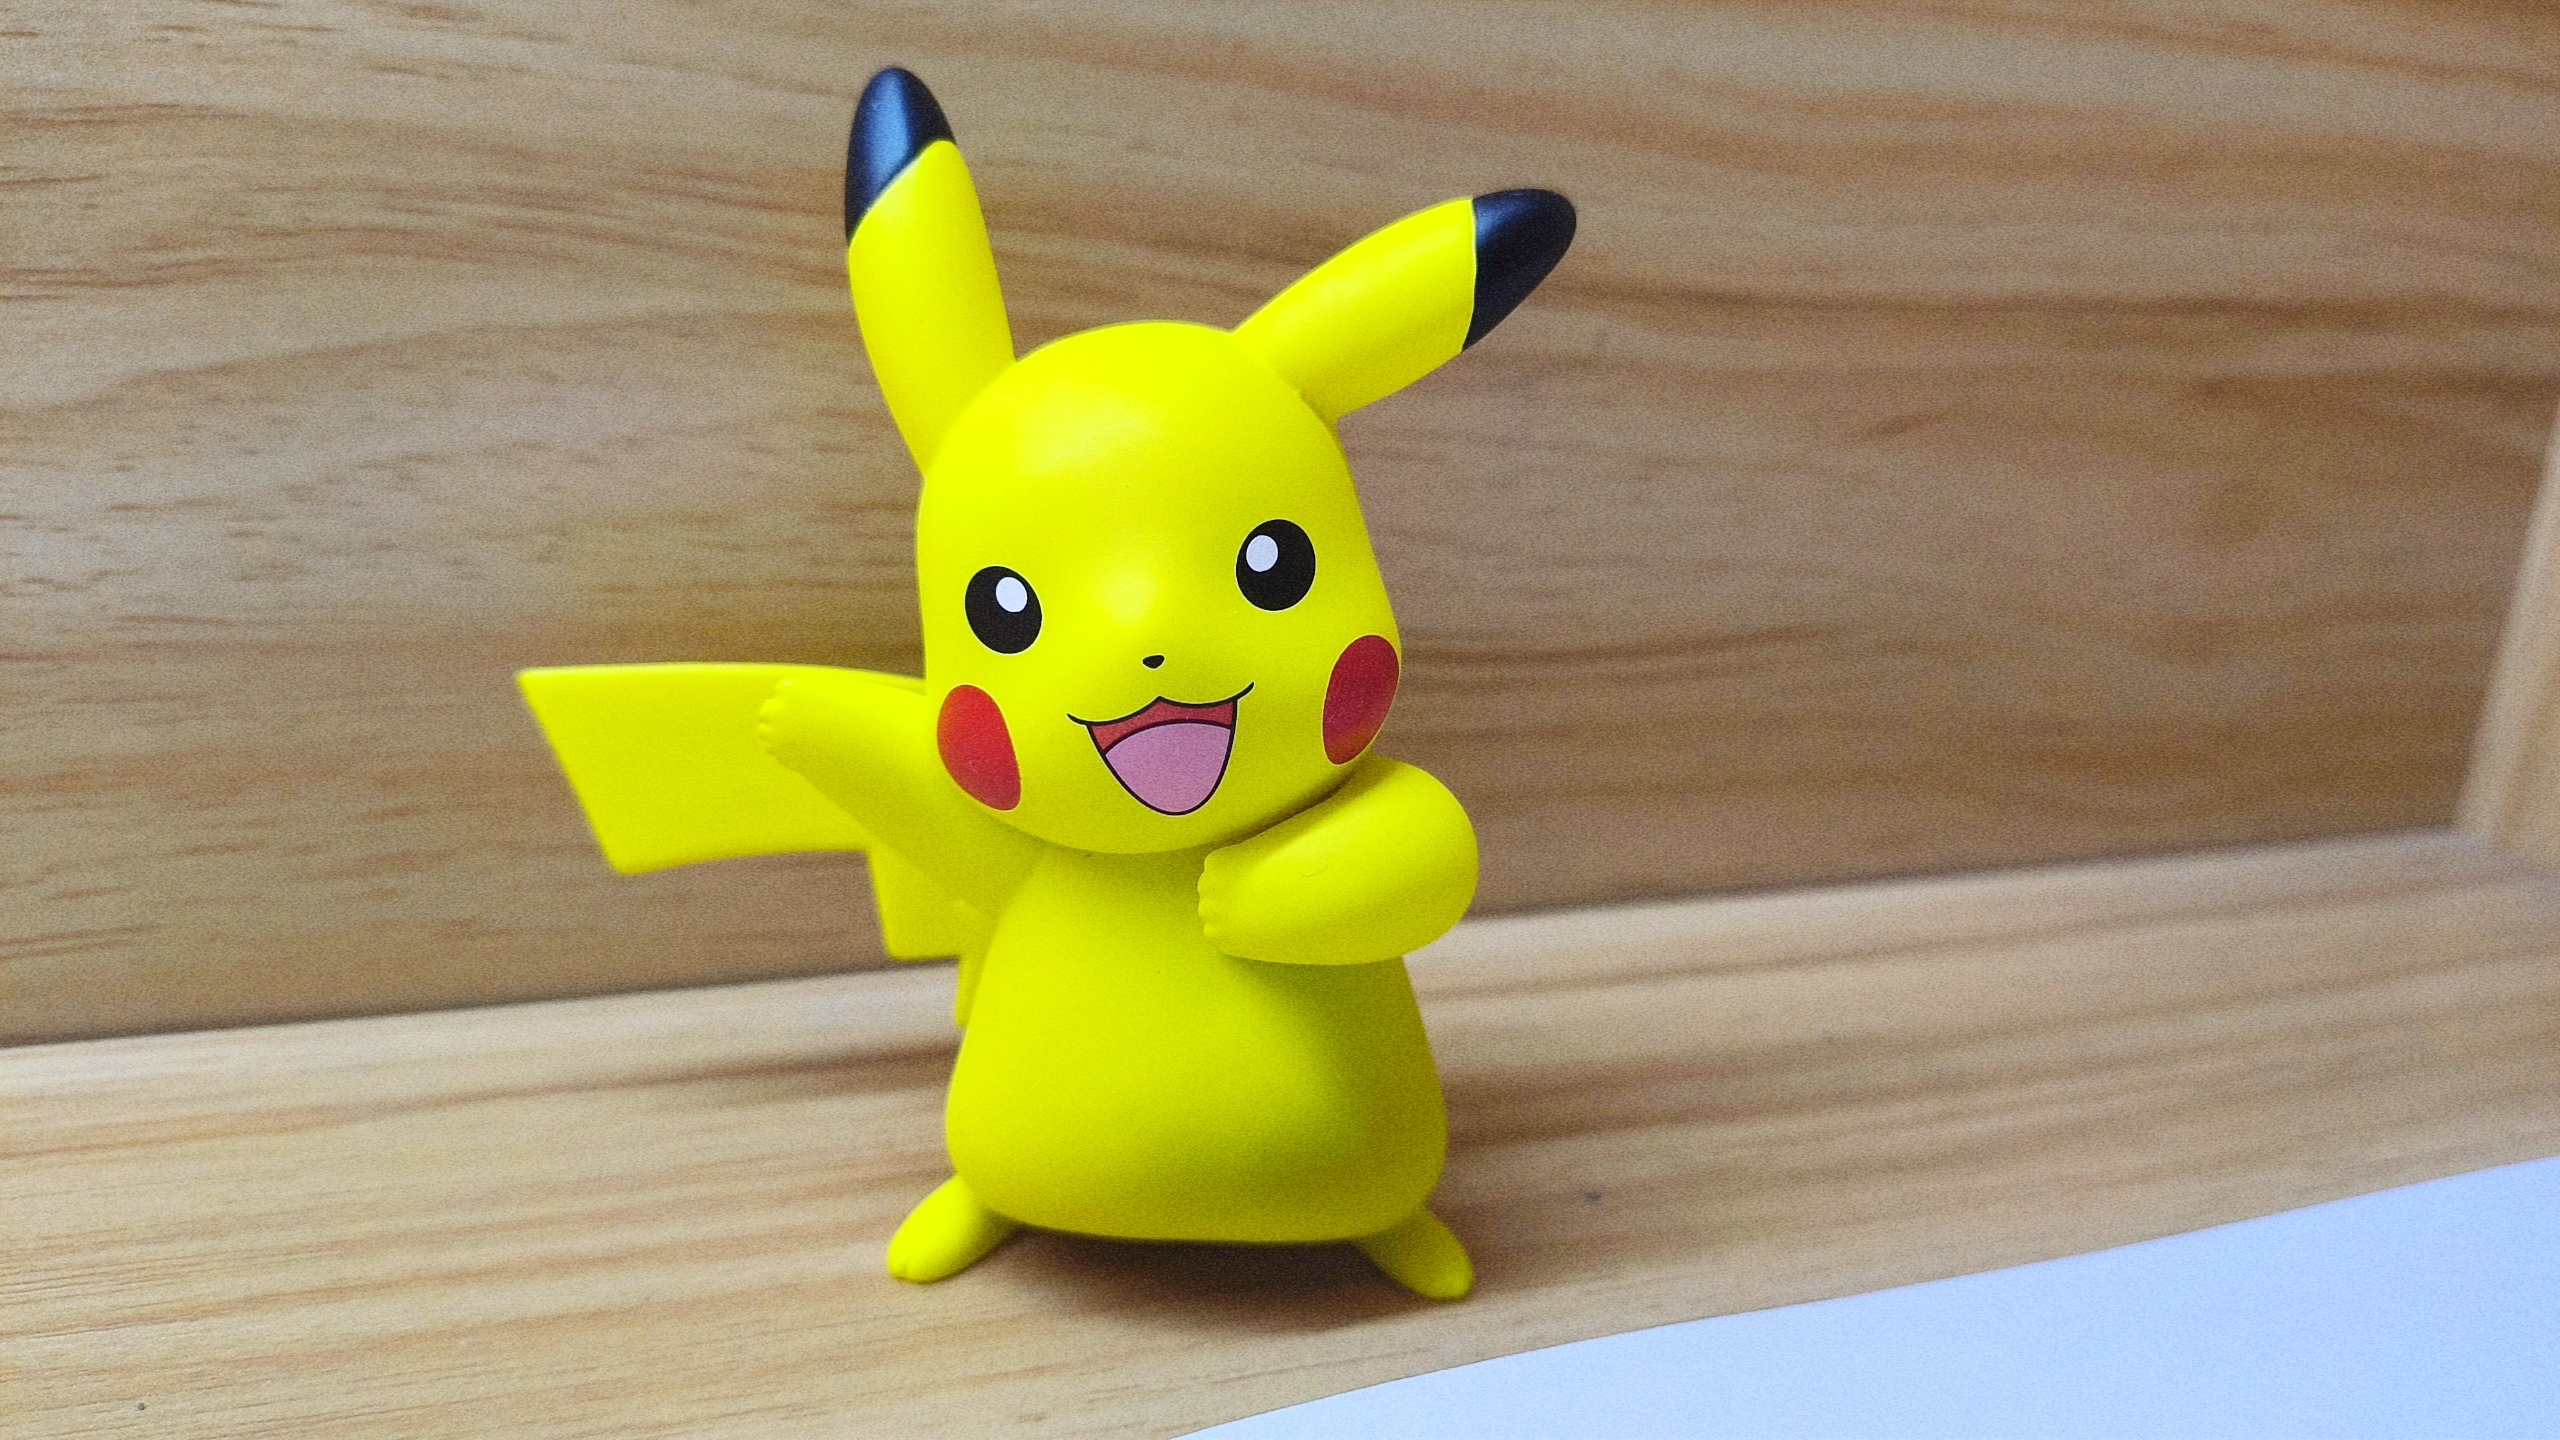
\includegraphics[scale=0.1]{figures/pikachu.jpg}
        \caption{这是图片}
        \label{fig:1}
    \end{figure}
    \begin{figure}[htbp]
        \centering
        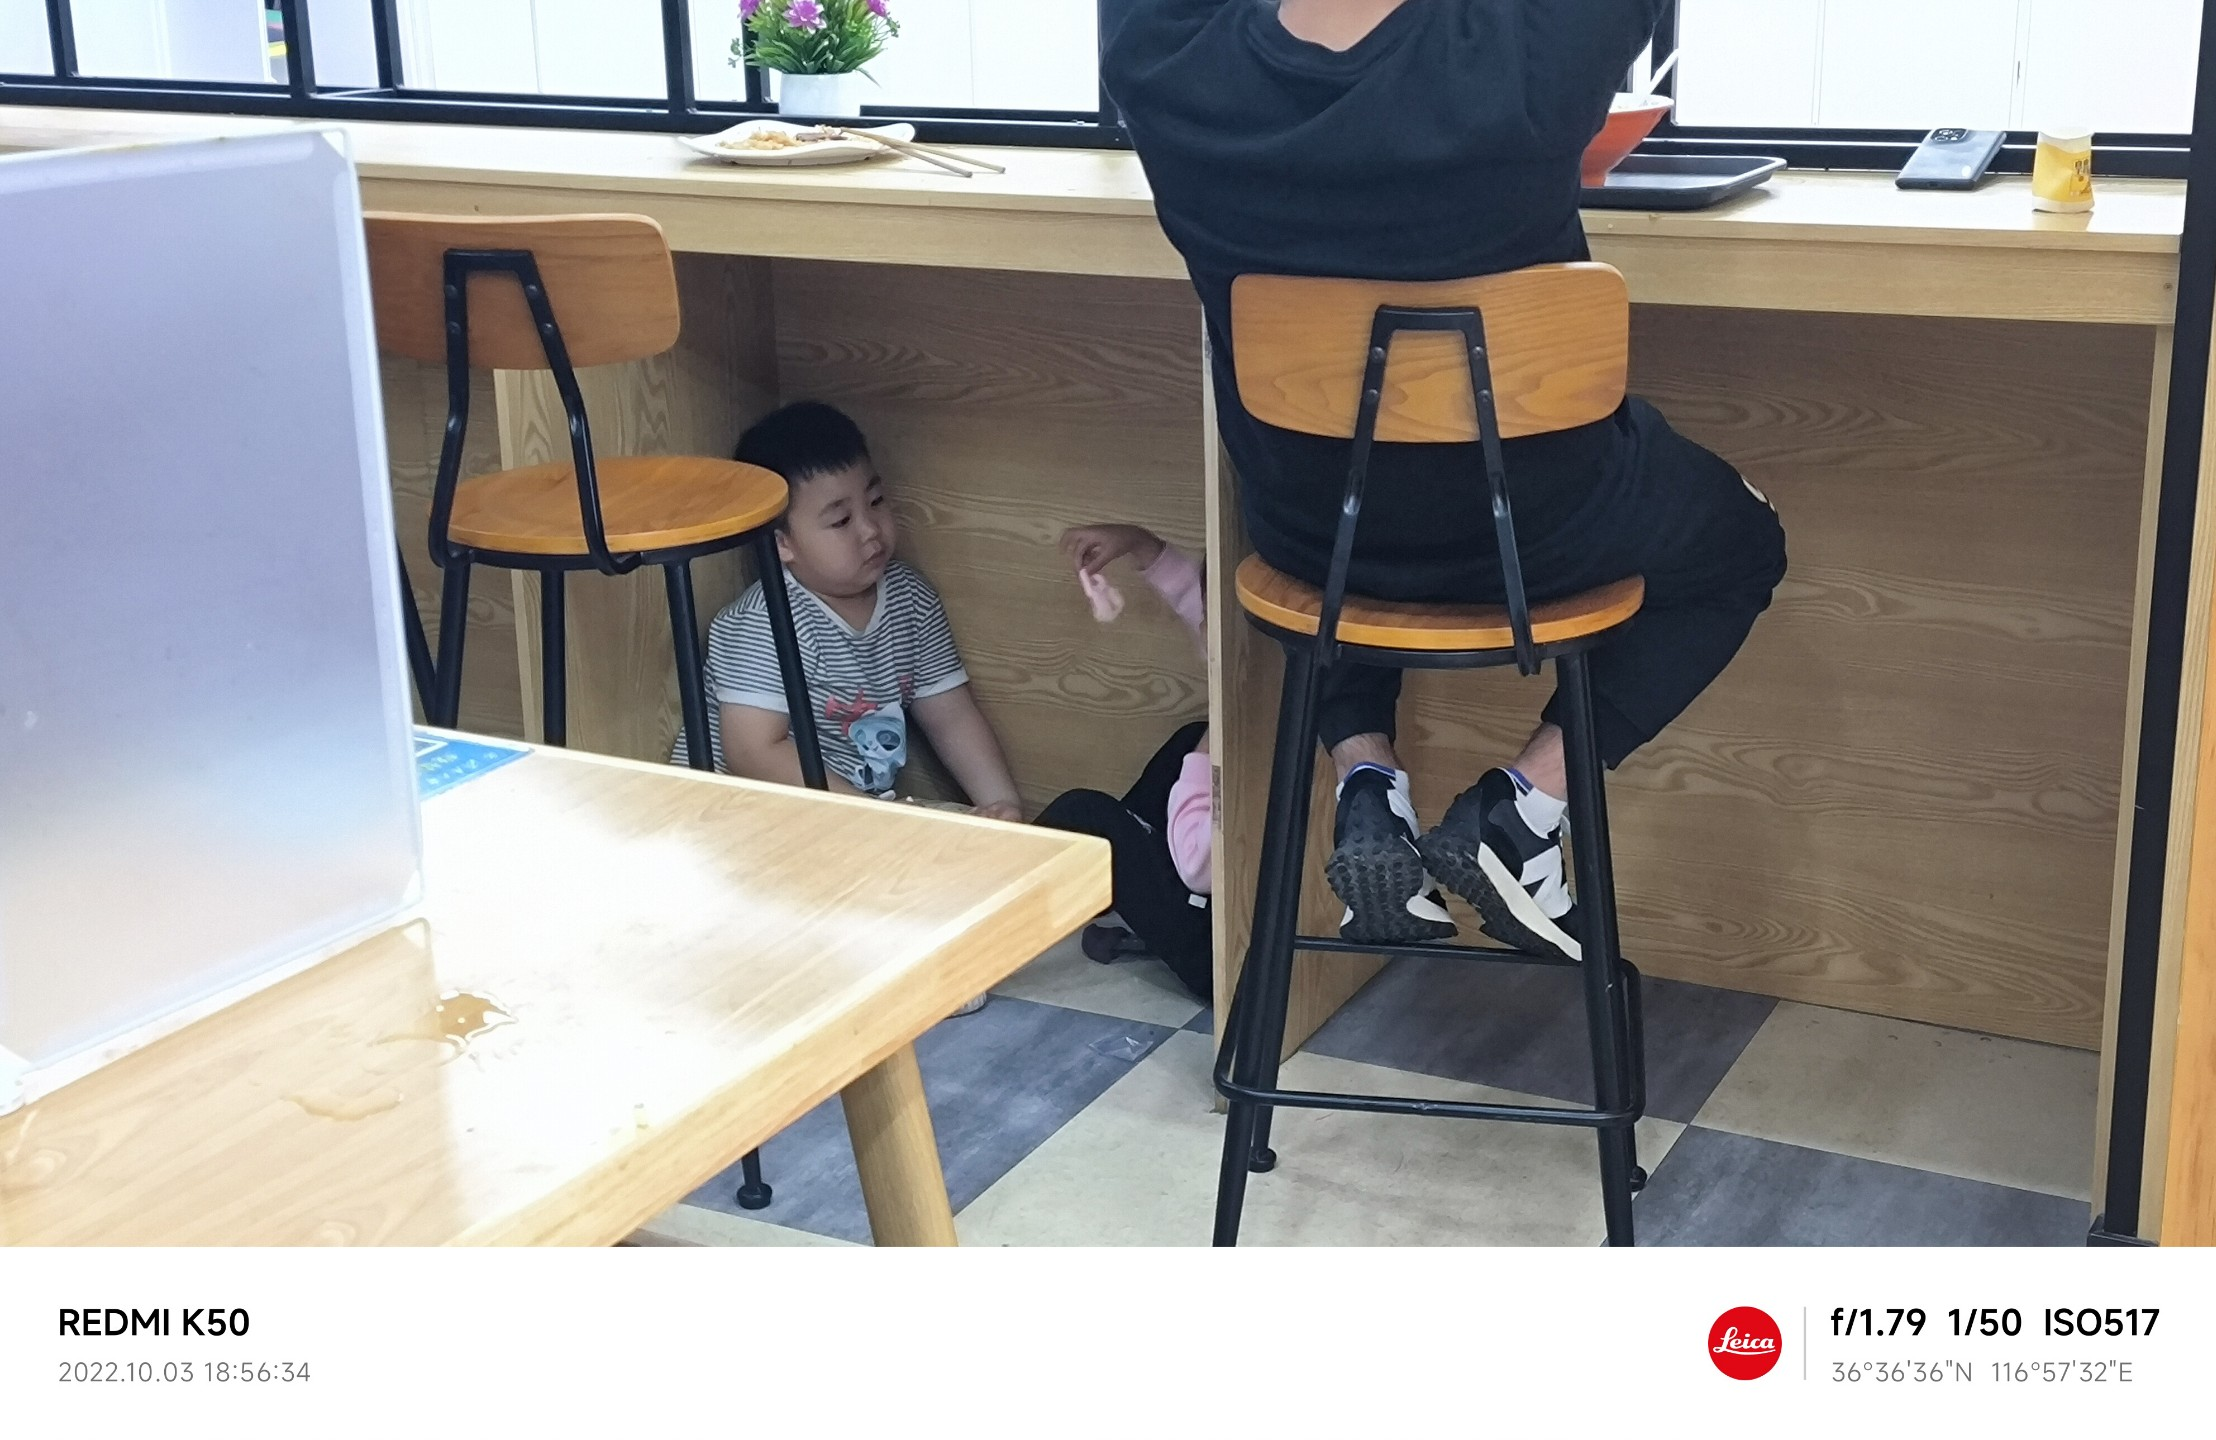
\includegraphics[scale=0.1]{figures/children.jpg}
        \caption{这是图片}
        \label{fig:2}
    \end{figure}
    \begin{figure}[htbp]
        \centering
        \includesvg[scale=1]{figures/latex-project-logo.svg}
        \caption{这是SVG图片(授权CC BY 4.0)}
        \label{fig:latex-project-logo}
      \end{figure}
    \subsubsection{表格}
    \begin{table}[!htbp]
        \centering
        \caption{这是表格}
        \begin{tabular}{cccccc}
            \toprule
            序号 & 姓名 & 性别 & 年龄 & 身高/cm & 体重/kg \\
            \midrule
            1 & 张三 & M & 16 & 163 & 50 \\
            2 & 王红 & F & 15 & 159 & 47 \\
            3 & 李二 & M & 17 & 165 & 52 \\
            \bottomrule
        \end{tabular}
        \label{tab:1}
    \end{table}
    % https://tex.stackexchange.com/questions/313625/latex-error-illegal-character-in-array-arg-table-parameter-mwidth
    \begin{table}[!htbp]
        \centering
        \caption{这是可限制列宽的表格}
        \begin{tabular}{c m{5cm}}
            \toprule
            类型 & 摘要 \\
            \midrule
            SHA256 & 7c240be293a091f20c202ac8e252d27b563cb78589ab7b340318234663d0dcf7 \\
            SHA512 & cb5cf3e1eb5e639a506a19a6585beae6dc4da57489ce296ab2272780b7317c13e6a76ca6c2bba94d0f475ca61ab4dff4b307636e2b1eb368b9508e37136e3fd8 \\
            单元格换行测试 & 李二 \newline 165 \newline 52 \\
            \bottomrule
        \end{tabular}
        \label{tab:2}
    \end{table}
    \subsection{交叉引用}\label{sec:1}
    \subsubsection{参考文献引用}\label{sec:2}
    首先引用一下大名鼎鼎的香农信息论\cite{shannon1948mathematical},所以哪能少得了图灵\cite{turing2009computing},因为看过《美丽心灵》就还有纳什\cite{nash1996non}。
    \subsubsection{图表引用}
    图片\ref{fig:1}和表格\ref{tab:1}的交叉引用。
    \subsubsection{章节引用}
    章节\ref{sec:1}和章节\ref{sec:2}的交叉引用。
    \subsubsection{公式引用}
    公式\ref{eq:1}的交叉引用。
    \subsubsection{Url引用}
    一个不算长也不算短但是必须得能自动换行的Url:\url{https://www.apple.com.cn/retail/parc66jinan/}
    \section{功能测试(节标题section)}
    \subsection{文字与段落(子节标题subsection)}
    这是文字。
    \subsubsection{段落(子小节标题subsubsection)}
    这是段落。这是段落。这是段落。这是段落。这是段落。这是段落。这是段落。这是段落。这是段落。这是段落。这是段落。这是段落。这是段落。这是段落。这是段落。这是段落。这是段落。这是段落。这是段落。这是段落。

    这是另一个段落。这是另一个段落。这是另一个段落。这是另一个段落。这是另一个段落。这是另一个段落。这是另一个段落。这是另一个段落。这是另一个段落。这是另一个段落。这是另一个段落。这是另一个段落。这是另一个段落。
    \subsection{数学公式}
    \subsubsection{行内公式}
    这是简单的行内公式:$x^2+y^2=z^2$,这是复杂的行内公式:$\sum_{i=1}^n a_i=0$。
    \subsubsection{行间公式}
    (1)线性代数:
    \begin{equation}
        \begin{split}
            \mathbf{A}^{-1} &= \frac{1}{\det(\mathbf{A})}\mathbf{A}^* \\
            \mathbf{A}^* &= \begin{bmatrix}
                \mathbf{A}_{11}^* & \mathbf{A}_{12}^* & \cdots & \mathbf{A}_{1n}^* \\
                \mathbf{A}_{21}^* & \mathbf{A}_{22}^* & \cdots & \mathbf{A}_{2n}^* \\
                \vdots & \vdots & \ddots & \vdots \\
                \mathbf{A}_{m1}^* & \mathbf{A}_{m2}^* & \cdots & \mathbf{A}_{mn}^*
            \end{bmatrix} \\
        \end{split}
    \end{equation}

    (2)微积分:
    \begin{equation}
        \begin{split}
            \frac{d}{dx}f(x) &= \lim_{h \to 0}\frac{f(x+h)-f(x)}{h} \\
            \frac{d^2}{dx^2}f(x) &= \lim_{h \to 0}\frac{f(x+h)-2f(x)+f(x-h)}{h^2} \\
            \frac{d^n}{dx^n}f(x) &= \lim_{h \to 0}\frac{f(x+h)-f(x)-\cdots-f(x-(n-1)h)}{h^n}
        \end{split}
        \label{eq:2}
    \end{equation}

    (3)概率论与数理统计:
    \begin{equation}
        \begin{split}
            P(A) &= \frac{\text{事件A发生的次数}}{\text{总次数}} \\
            P(A \mid B) &= \frac{P(A \cap B)}{P(B)} \\
            P(A \cap B) &= P(A)P(B \mid A) \\
            P(A \cup B) &= P(A) + P(B) - P(A \cap B)
        \end{split}
    \end{equation}

    \begin{equation}
        \begin{split}
            E(X) &= \sum_{i=1}^n x_iP(X=x_i) \\
            E(XY) &= \sum_{i=1}^n \sum_{j=1}^n x_iy_jP(X=x_i,Y=y_j) \\
            E(X \mid Y) &= \sum_{i=1}^n x_iP(X=x_i \mid Y=y) \\
            E(X \mid Y=y) &= \sum_{i=1}^n x_iP(X=x_i,Y=y) \\
            E(X \mid Y=y_1,y_2,\cdots,y_k) &= \sum_{i=1}^n x_iP(X=x_i,Y=y_1,Y=y_2,\cdots,Y=y_k)
        \end{split}
    \end{equation}

    (4)数学分析:

    \begin{equation}
        \begin{split}
            \lim_{x \to a}f(x) &= L \\
            \lim_{x \to a^+}f(x) &= L \\
            \lim_{x \to a^-}f(x) &= L \\
            \lim_{x \to a^+}f(x) &= \lim_{x \to a^-}f(x) \\
            \lim_{x \to a^+}f(x) &= \lim_{x \to a^-}f(x) = L
        \end{split}
    \end{equation}

    (5)离散数学:
    \begin{equation}
        \begin{split}
            \binom{n}{k} &= \frac{n!}{k!(n-k)!} \\
            \binom{n}{0} &= \binom{n}{n} = 1 \\
            \binom{n}{1} &= \binom{n}{n-1} = n \\
            \binom{n}{2} &= \binom{n}{n-2} = \frac{n(n-1)}{2}
        \end{split}
    \end{equation}

    (6)复变函数:
    \begin{equation}
        \begin{split}
            \lim_{z \to \infty}f(z) &= L \\
            \lim_{z \to \infty}f(z) &= \lim_{z \to -\infty}f(z) \\
            \lim_{z \to \infty}f(z) &= \lim_{z \to -\infty}f(z) = L \\
            \lim_{z \to \infty}f(z) &= \lim_{z \to -\infty}f(z) \neq L
        \end{split}
    \end{equation}
    \subsection{代码块与图表}
    \subsubsection{代码块}
    \begin{lstlisting}[language=C]
        #include <stdio.h>
        /* hello,world */
        int main(){
            printf("Hello, World! \n"); 
            return 0;
        }
    \end{lstlisting}
    \subsubsection{图片}
    \begin{figure}[htbp]
        \centering
        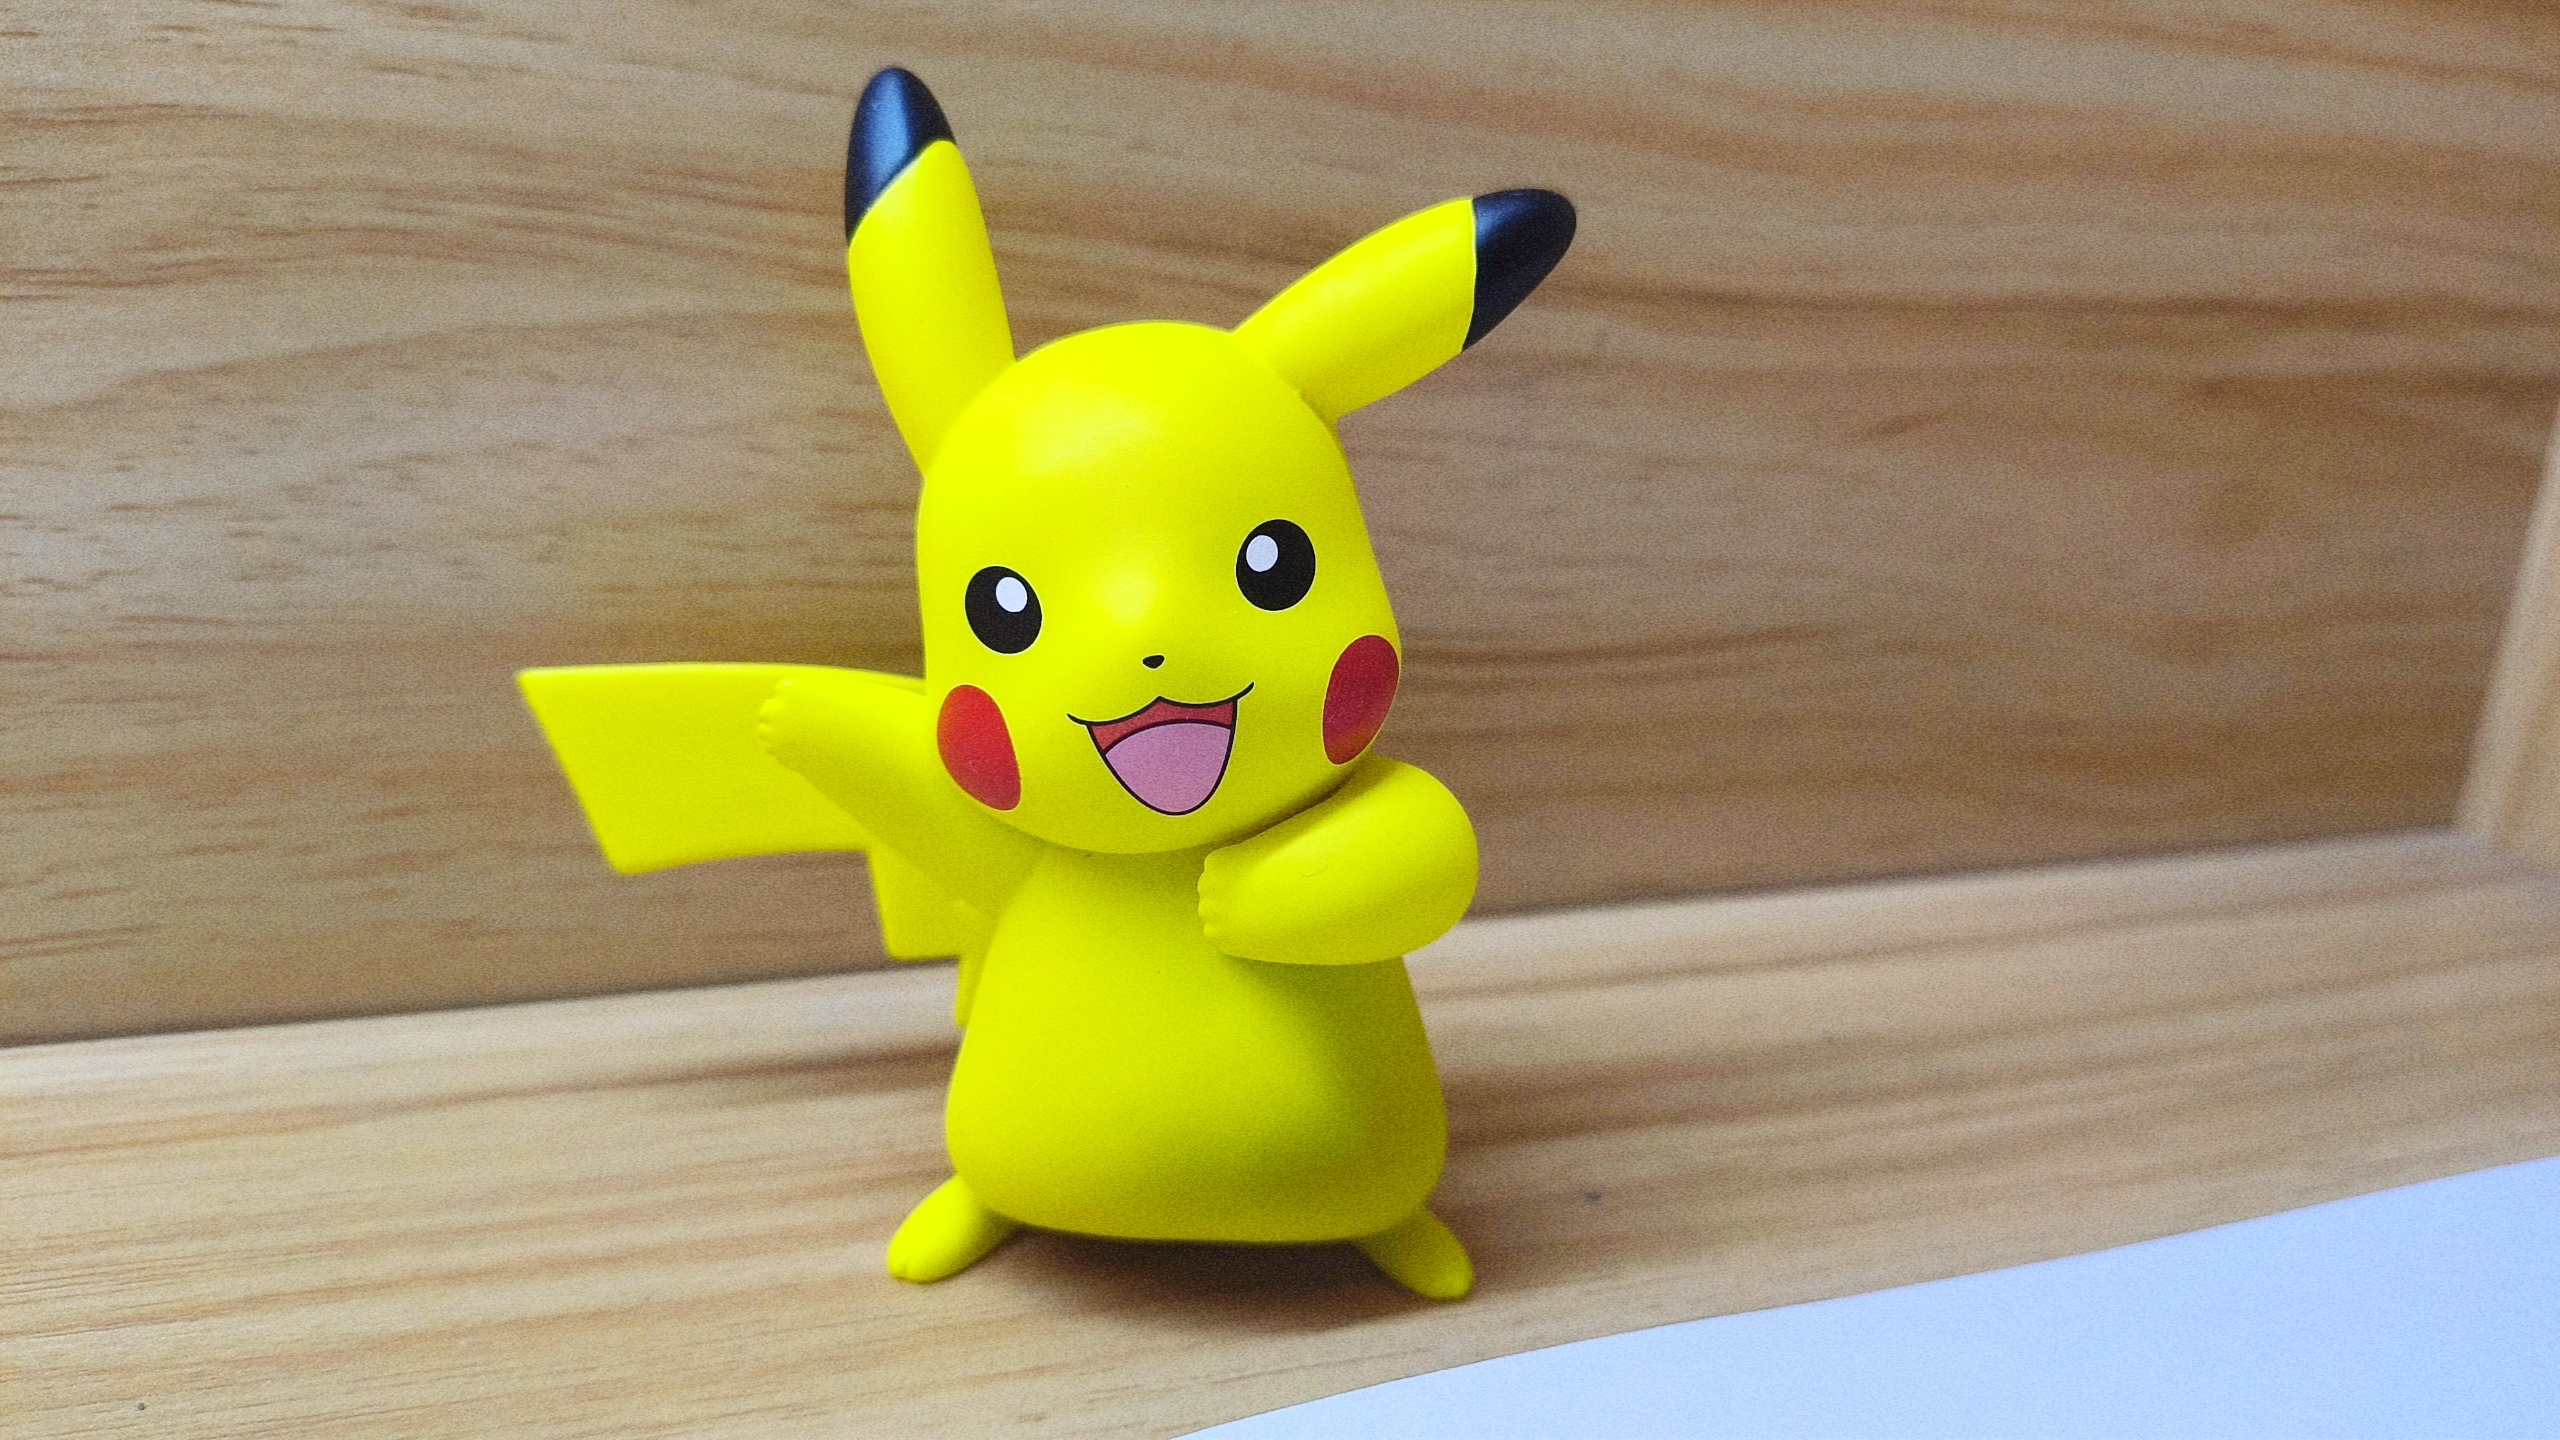
\includegraphics[scale=0.1]{figures/pikachu.jpg}
        \caption{这是图片}
        \label{fig:3}
    \end{figure}
    \begin{figure}[htbp]
        \centering
        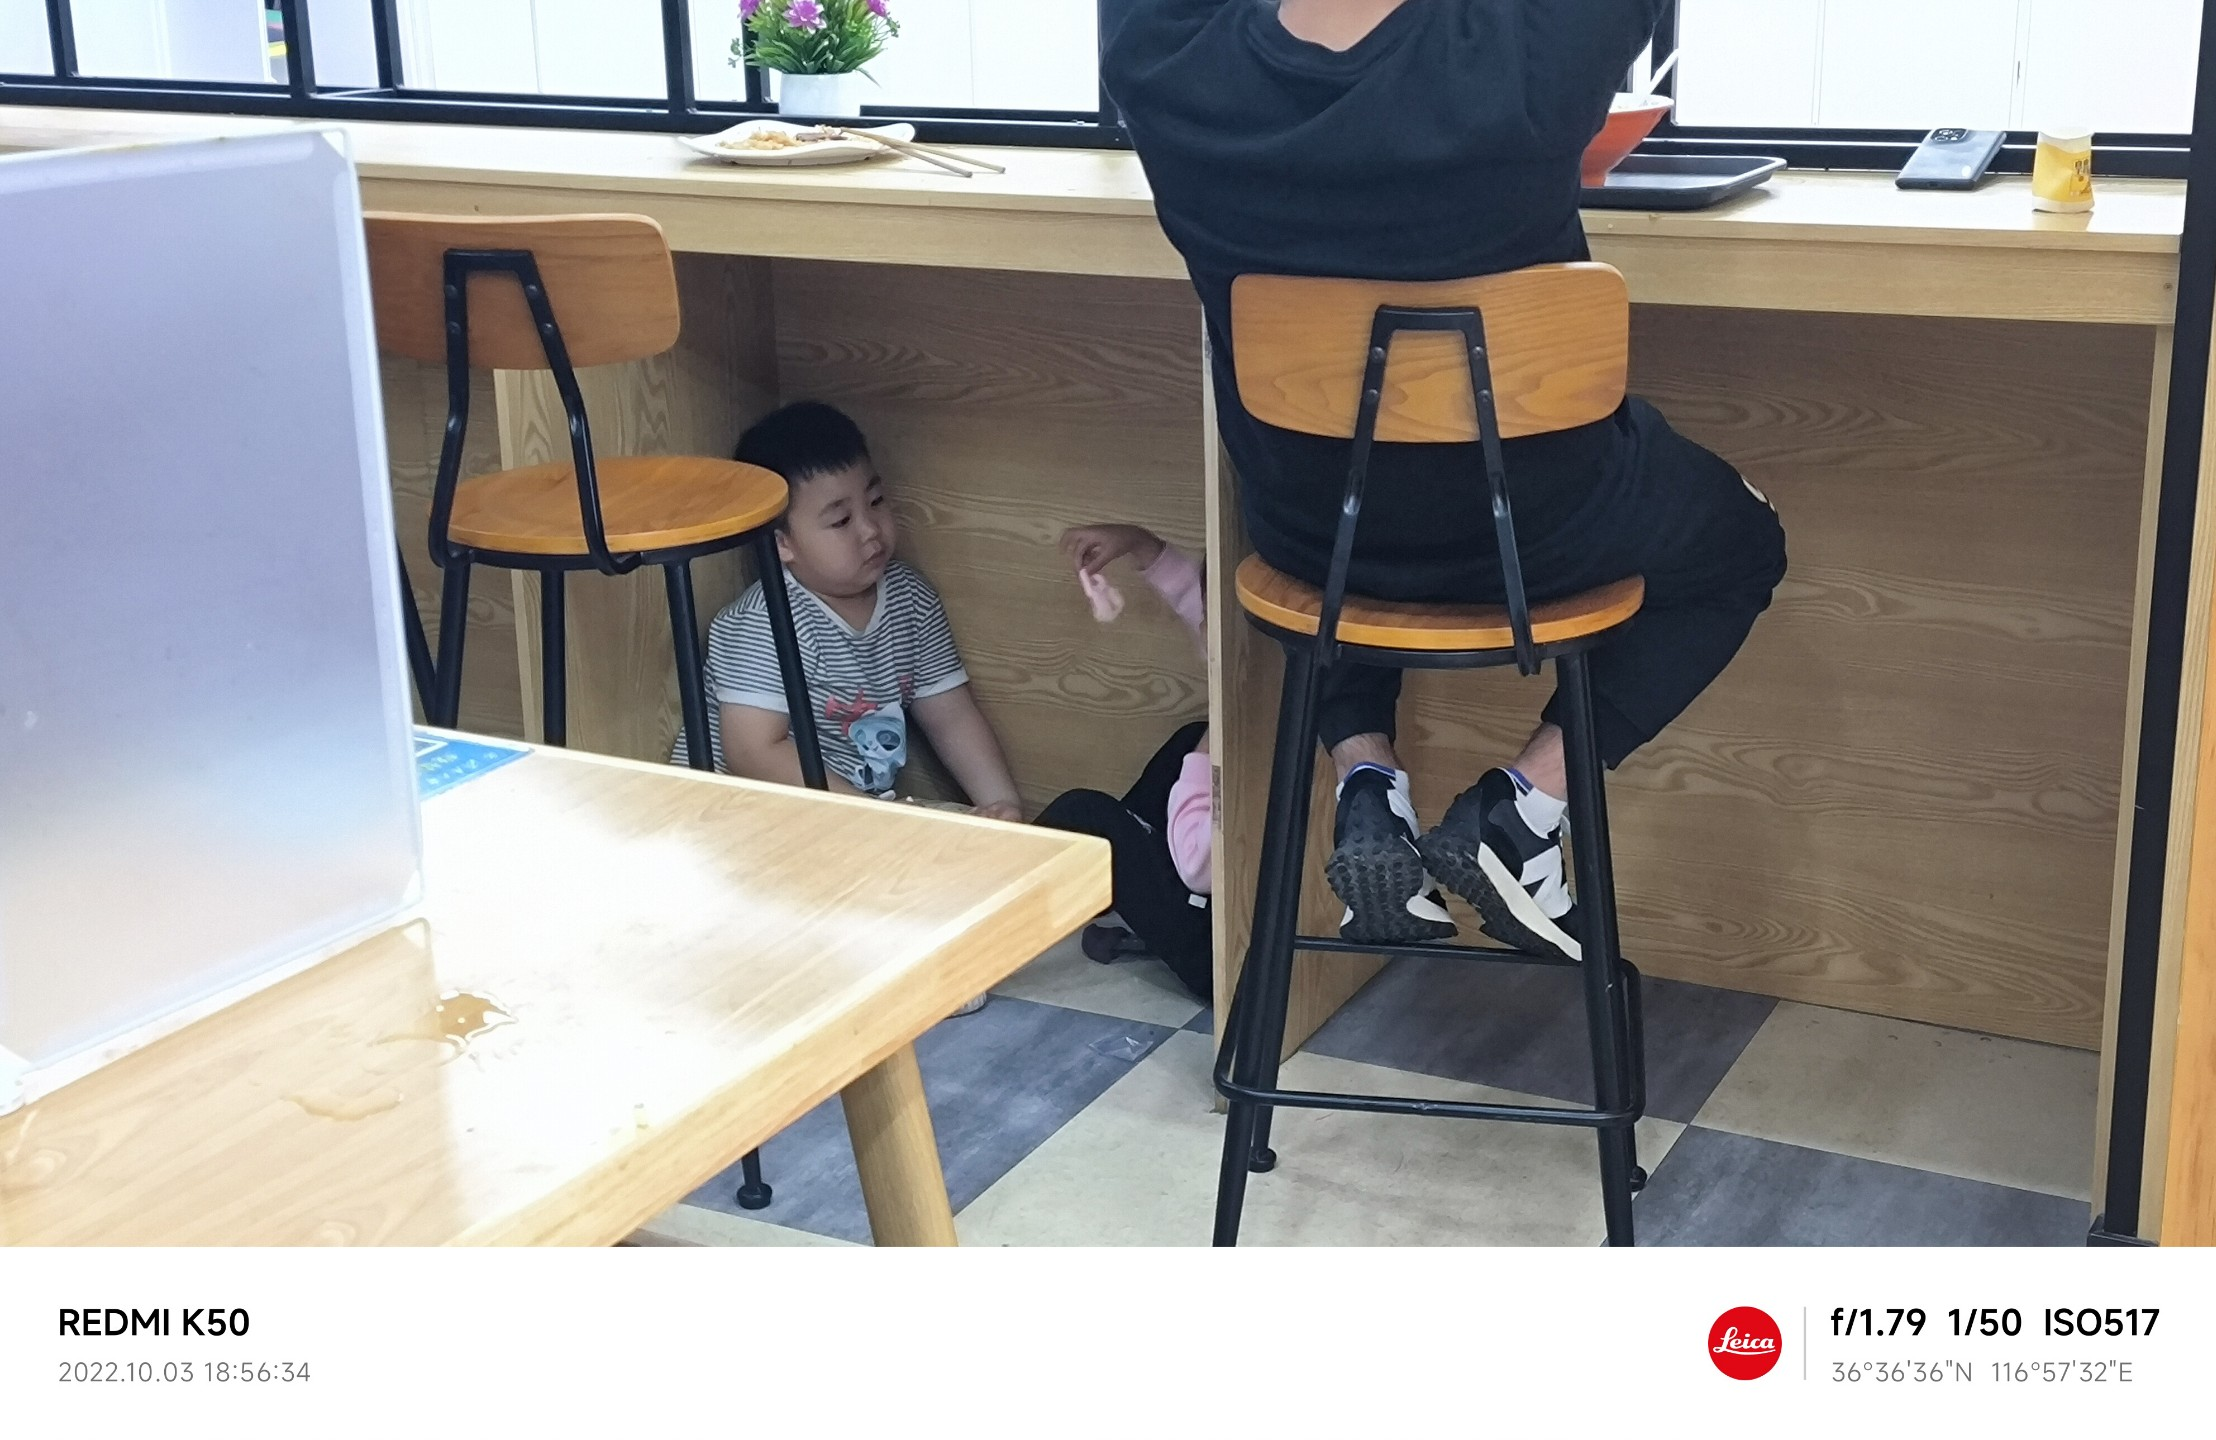
\includegraphics[scale=0.1]{figures/children.jpg}
        \caption{这是图片}
        \label{fig:4}
    \end{figure}
    \subsubsection{表格}
    \begin{table}[!htbp]
        \centering
        \caption{这是表格}
        \begin{tabular}{cccccc}
            \toprule
            序号 & 姓名 & 性别 & 年龄 & 身高/cm & 体重/kg \\
            \midrule
            1 & 张三 & M & 16 & 163 & 50 \\
            2 & 王红 & F & 15 & 159 & 47 \\
            3 & 李二 & M & 17 & 165 & 52 \\
            \bottomrule
        \end{tabular}
        \label{tab:2}
    \end{table}
    \subsection{交叉引用}\label{sec:3}
    \subsubsection{参考文献引用}\label{sec:4}
    首先引用一下大名鼎鼎的香农信息论\cite{shannon1948mathematical},所以哪能少得了图灵\cite{turing2009computing},因为看过《美丽心灵》就还有纳什\cite{nash1996non}。
    \subsubsection{图表引用}
    图片\ref{fig:2}和表格\ref{tab:2}的交叉引用。
    \subsubsection{章节引用}
    章节\ref{sec:3}和章节\ref{sec:4}的交叉引用。
    \subsubsection{公式引用}
    公式\ref{eq:2}的交叉引用。
    \subsubsection{Url引用}
    一个不算长也不算短但是必须得能自动换行的Url:\url{https://www.apple.com.cn/retail/parc66jinan/}
% ·································································································
\end{ujnbody}                        % 2.4 正文

\pagestyle{ujnothers}
\begin{ujnconclusion}
\section[结论]{结\qquad 论}
% 以下为结论,把点引线以下的文字替换成你的就好
% ·································································································
(1)总而言之,言而总之,这篇论文结束了,至于写了什么,反正就是写了一些东西,然后就结束了,这就是结论,我随便写写,你随便看看。

(2)总而言之,言而总之,这篇论文结束了,至于写了什么,反正就是写了一些东西,然后就结束了,这就是结论,我随便写写,你随便看看。

(3)总而言之,言而总之,这篇论文结束了,至于写了什么,反正就是写了一些东西,然后就结束了,这就是结论,我随便写写,你随便看看。
% ·································································································
\end{ujnconclusion}
                  % 2.5 结论
% 一般来说,这里不需要修改
\begin{ujnreference}
\addcontentsline{toc}{section}{参考文献}
\small
\bibliographystyle{gbt7714-2005}
\bibliography{ref}
\end{ujnreference}
                   % 2.6 参考文献
\begin{ujnthanks}
\section[致谢]{致\qquad 谢}
% 以下为致谢,把点引线以下的文字替换成你的就好
% ·································································································
讲三句话:

(1)对毕业论文写作成功致以热烈的祝贺。

(2)向论文写作过程中对我论文写作成功作出过帮助的师长,同时向社会各界帮助我论文写作的朋友、向国际学术界友人,表示衷心的感谢。

(3)希望我同未来的同学、同事一起,奋发努力,扎实工作,把自己的小我向社会的大我融入成功。
% ·································································································
\end{ujnthanks}
                      % 2.7 致谢
\begin{ujnappendix}
\section[附录]{附\qquad 录}
% 以下为附录,把点引线以下的文字替换成你的就好
% ·································································································
    \subsection*{附录A 计算机的层次模型}
        \begin{figure}[htbp]
            \centering
            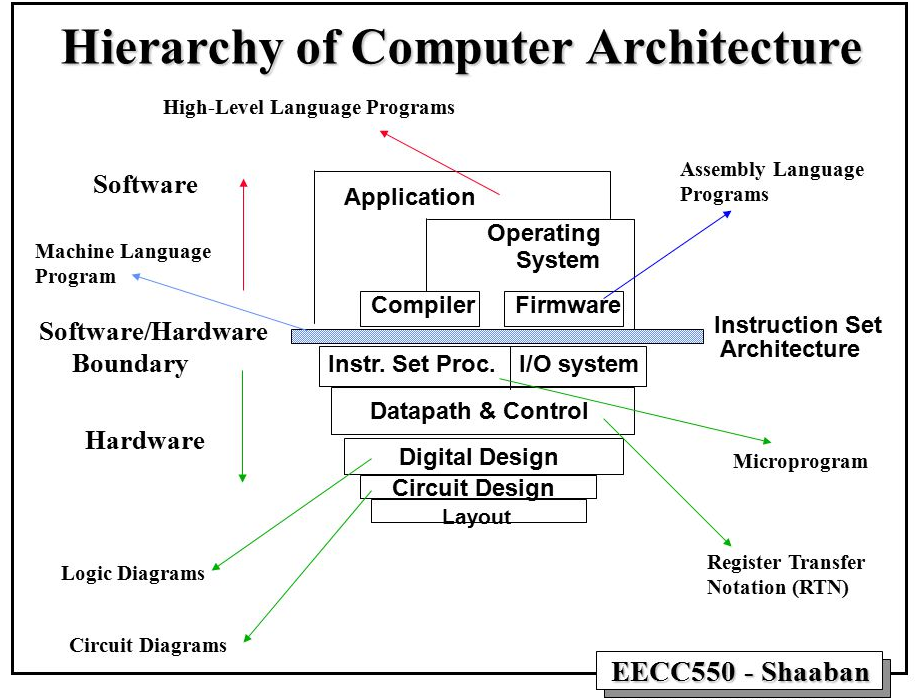
\includegraphics[width=0.8\textwidth]{figures/computer-arch.png}
            \caption{计算机的层次模型}
            \label{fig:computer-arch}
        \end{figure}
    \subsection*{附录B RV32I Base Integer Instruction Set}
% ·································································································
\end{ujnappendix}
                    % 2.8 附录
\unsetblindingline
\unsetfancylength

%%%%%%%%%%%%%%%%%%%%%%%%%%%%%% 毕业论文正文 %%%%%%%%%%%%%%%%%%%%%%%%%%%%%%%%%

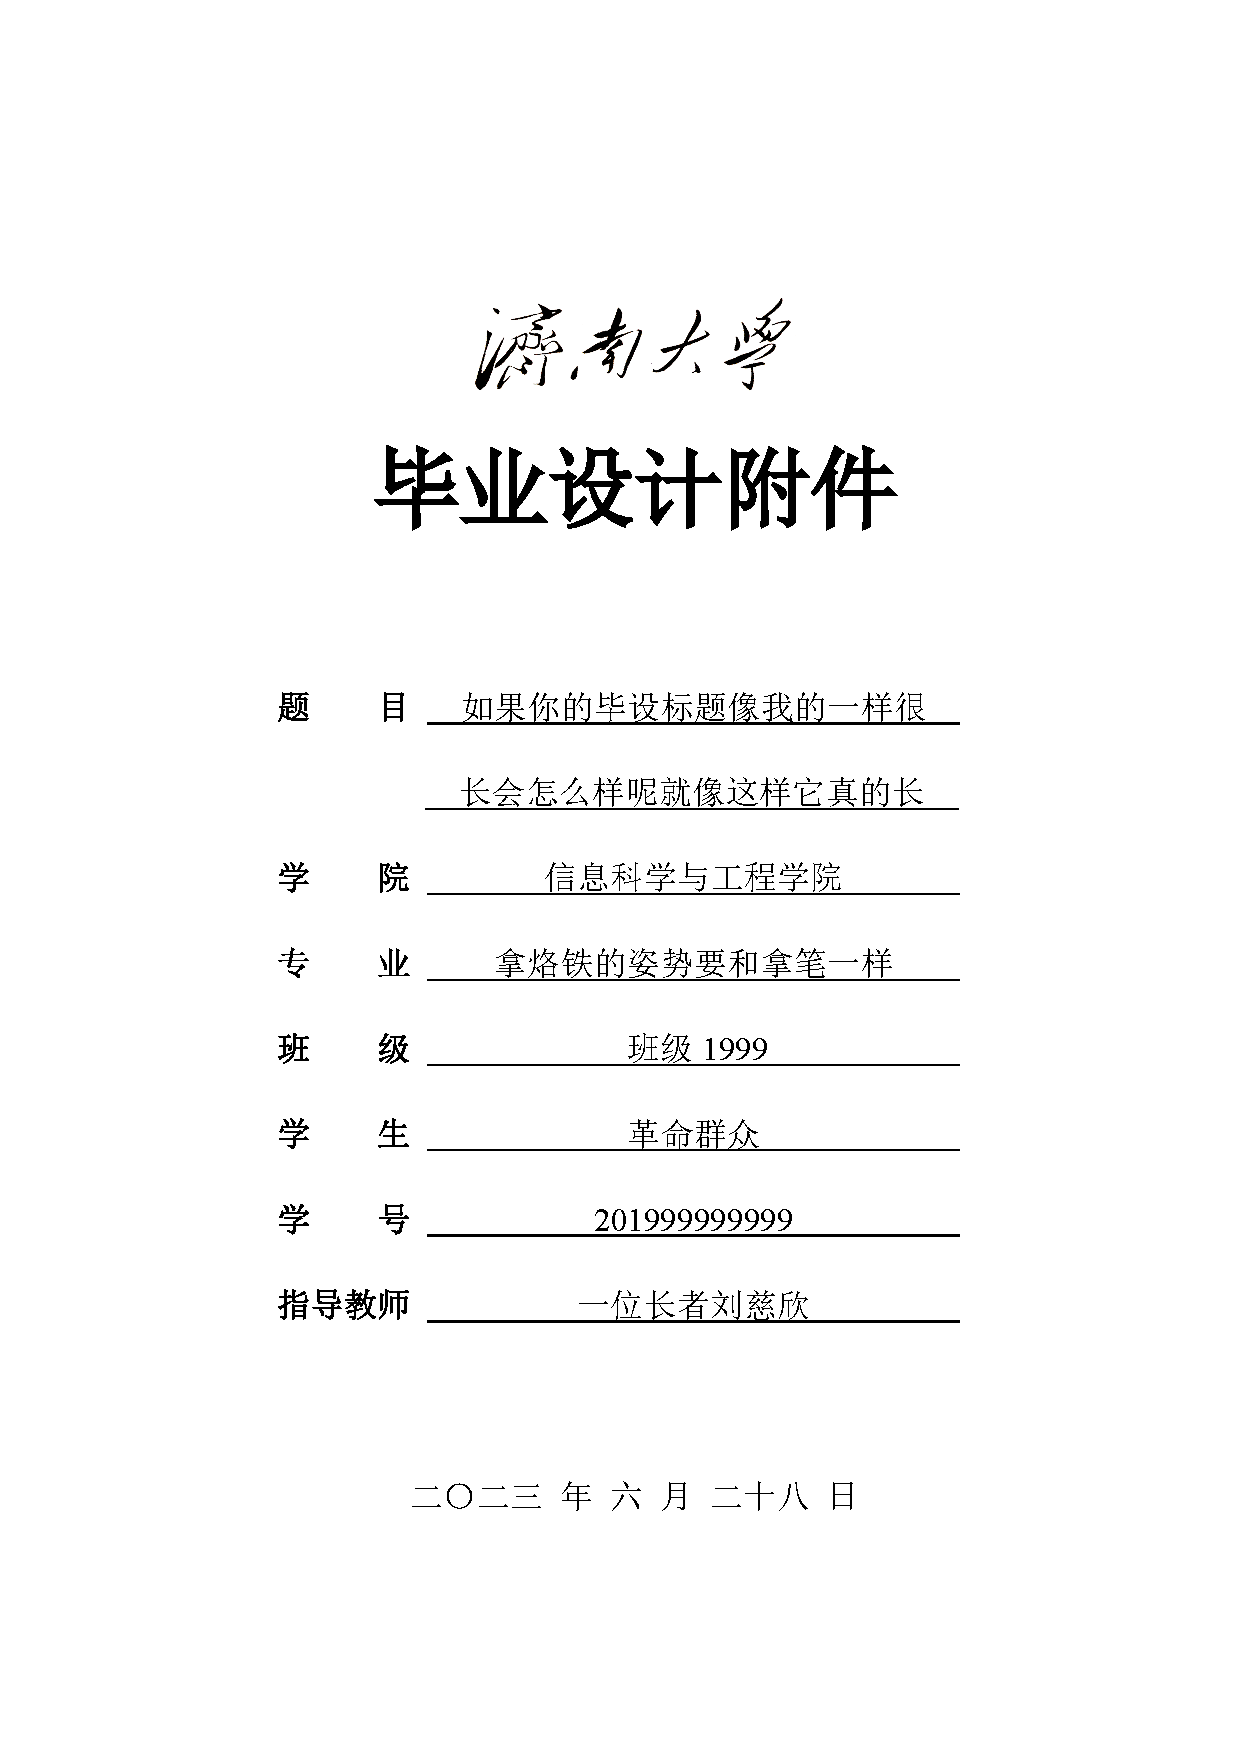
\includepdf[pages=-]{docs/03-appendix-cover.pdf}            % 3-6 表格性质的其他内容
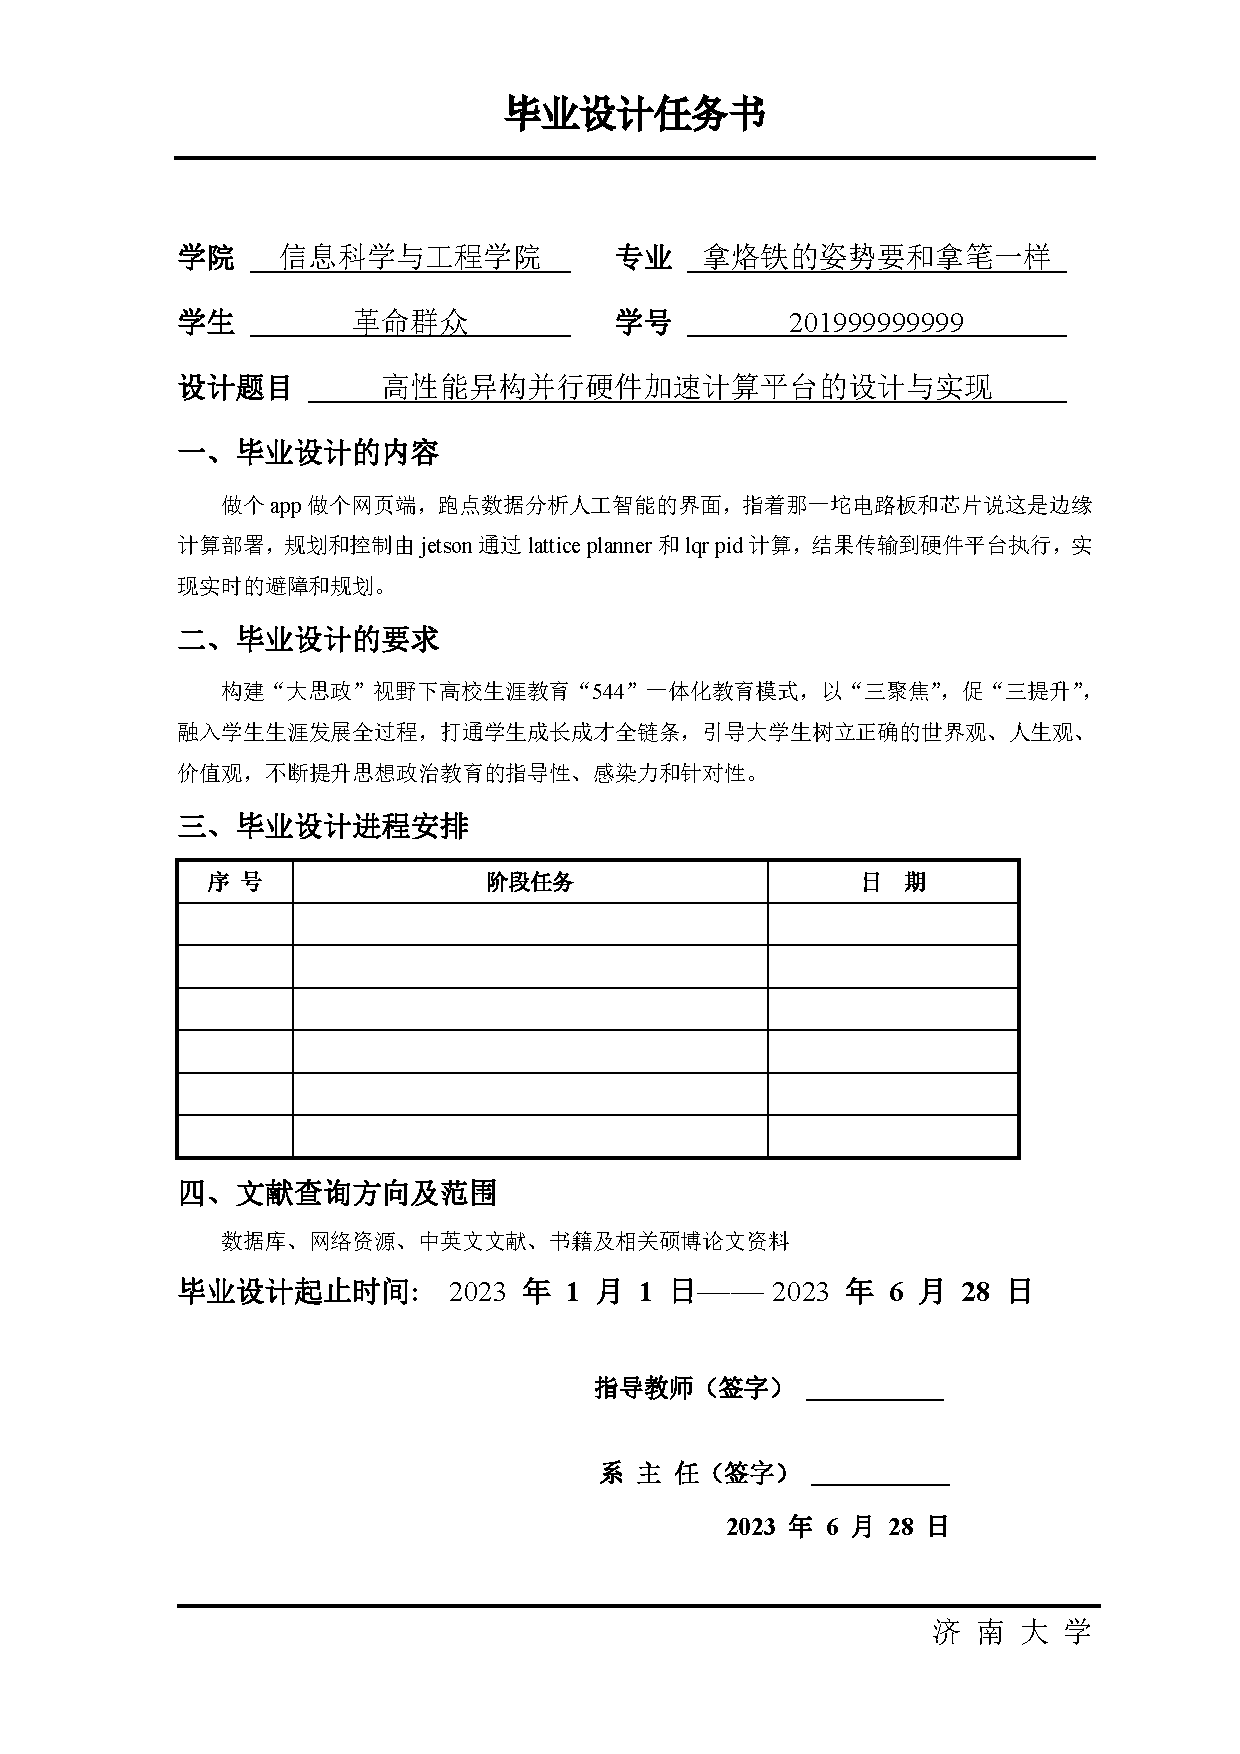
\includepdf[pages=-]{docs/04-taskbook.pdf}
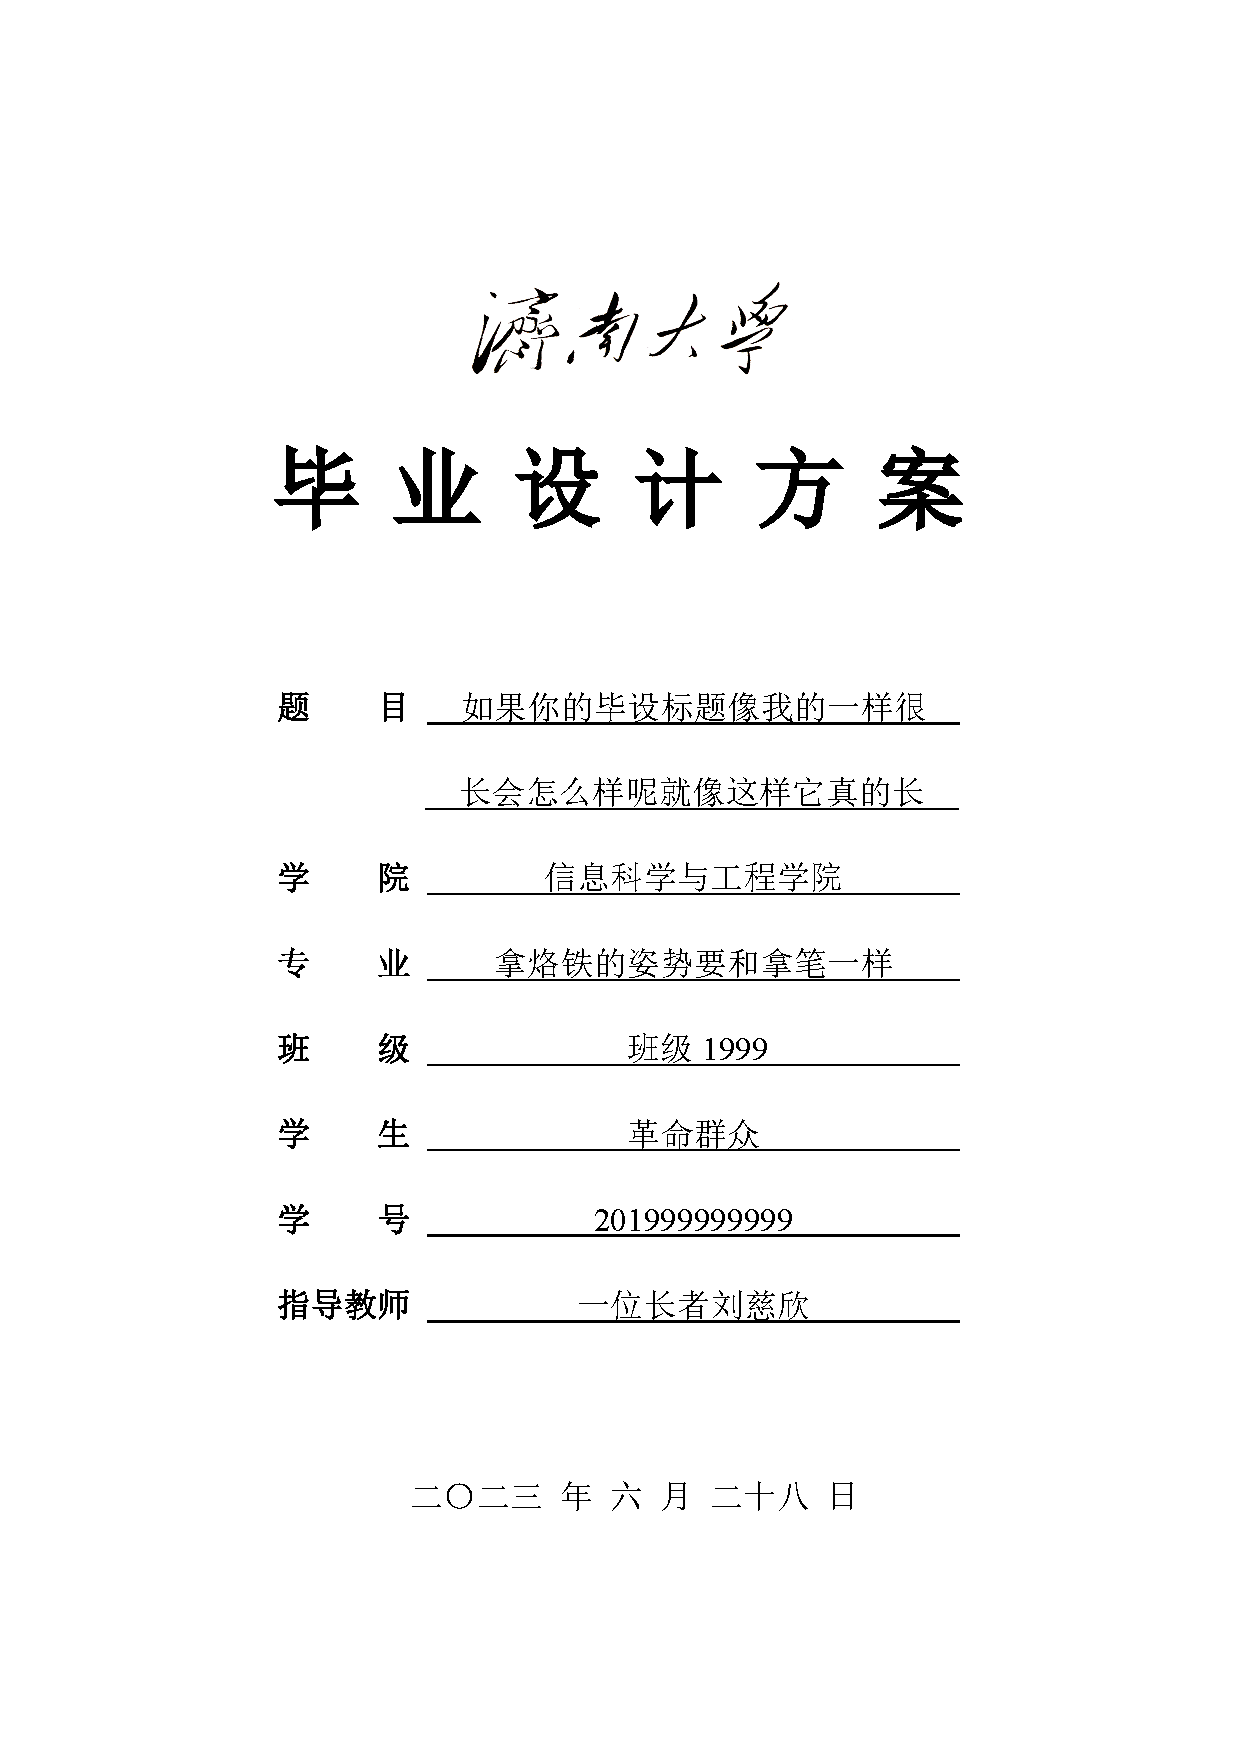
\includepdf[pages=-]{docs/05-report.pdf}

\end{document}
